\newpage
\section{Auswertung}
\label{sec:Auswertung}

\begin{table}
  \centering
  \caption{Temperatur und Druck bei Verdampfung des Wassers. Der Druck hat eine Messunsicherheit von
  $\pm$mB, die Temperatur von $\pm 1$ K.},
  \label{tab:Messreihe_1}
\begin{tabular}{
  c c||c c||c c||c c
}
\toprule 
$T/ \unit{\kelvin}$ & $p / \text{mB}$ & $T/ \unit{\kelvin}$ & $p / \text{mB}$&
$T/ \unit{\kelvin}$ & $p / \text{mB}$ & $T/ \unit{\kelvin}$ & $p / \text{mB}$ \\
\midrule
293,15  & 40   & 313,15  & 372  & 333,15  & 528  & 353,15  & 773 \\
294,15  & 167  & 314,15  & 379  & 334,15  & 537  & 354,15  & 790 \\
295,15  & 228  & 315,15  & 385  & 335,15  & 549  & 355,15  & 810 \\
296,15  & 255  & 316,15  & 395  & 336,15  & 562  & 356,15  & 826 \\
297,15  & 274  & 317,15  & 400  & 337,15  & 571  & 357,15  & 844 \\
298,15  & 287  & 318,15  & 405  & 338,15  & 578  & 358,15  & 856 \\
299,15  & 296  & 319,15  & 412  & 339,15  & 586  & 359,15  & 879 \\
300,15  & 303  & 320,15  & 421  & 340,15  & 600  & 360,15  & 901 \\
301,15  & 310  & 321,15  & 431  & 341,15  & \text{--}  & 361,15  & 913 \\
302,15  & 316  & 322,15  & 439  & 342,15  & 628  & 362,15  & 933 \\
303,15  & 322  & 323,15  & 445  & 343,15  & 638  & 363,15  & 944 \\
304,15  & 327  & 324,15  & 453  & 344,15  & 650  & 364,15  & 966 \\
305,15  & 331  & 325,15  & 461  & 345,15  & 660  & 365,15  & 979 \\
306,15  & 336  & 326,15  & 465  & 346,15  & 670  & 366,15  & 990 \\
307,15  & 341  & 327,15  & 476  & 347,15  & 690  & 367,15  & 1015\\
308,15  & 347  & 328,15  & 482  & 348,15  & 701  & 368,15  & 1030\\
309,15  & 351  & 329,15  & 491  & 349,15  & 716  & 369,15  & 1046\\
310,15  & 356  & 330,15  & 500  & 350,15  & 723  & 370,15  & 1061\\
311,15  & 362  & 331,15  & 511  & 351,15  & 743  & 371,15  & 1079\\
312,15  & 367  & 332,15  & 520  & 352,15  & 760  & 372,15  & 1093\\
      &   &       &       &       &      & 373,15  & 1108 \\
\bottomrule
\end{tabular}
\end{table}
\begin{table}
  \centering
  \caption{Temperatur und Druck bei Verdampfung des Wassers für $p\geq 1$.Der Druck hat eine Messunsicherheit von
  $\pm$mB, die Temperatur von $\pm 1$ K.},
  \label{tab:Messreihe_2}
\begin{tabular}{
  c c||c c
}
\toprule 
$p$/B & $T$/K & $p$/B & $T$/K\\
\midrule
1000  & 391,15 & 9000  & 447,15\\
2000  & 404,15 & 10000 & 451,15\\
3000  & 413,15 & 11000 & 454,15\\
4000  & 419,15 & 12000 & 459,15\\
5000  & 427,15 & 13000 & 461,15\\
6000  & 433,15 & 14000 & 463,15\\
7000  & 438,15 & 15000 & 465,15\\
8000  & 443,15 &       &       \\
\bottomrule
\end{tabular}
\end{table}

Mit diesen Messwerten lassen sich folgende Grafiken erstellen:
\begin{figure}[H]
  \begin{subfigure}{0.48\textwidth}
      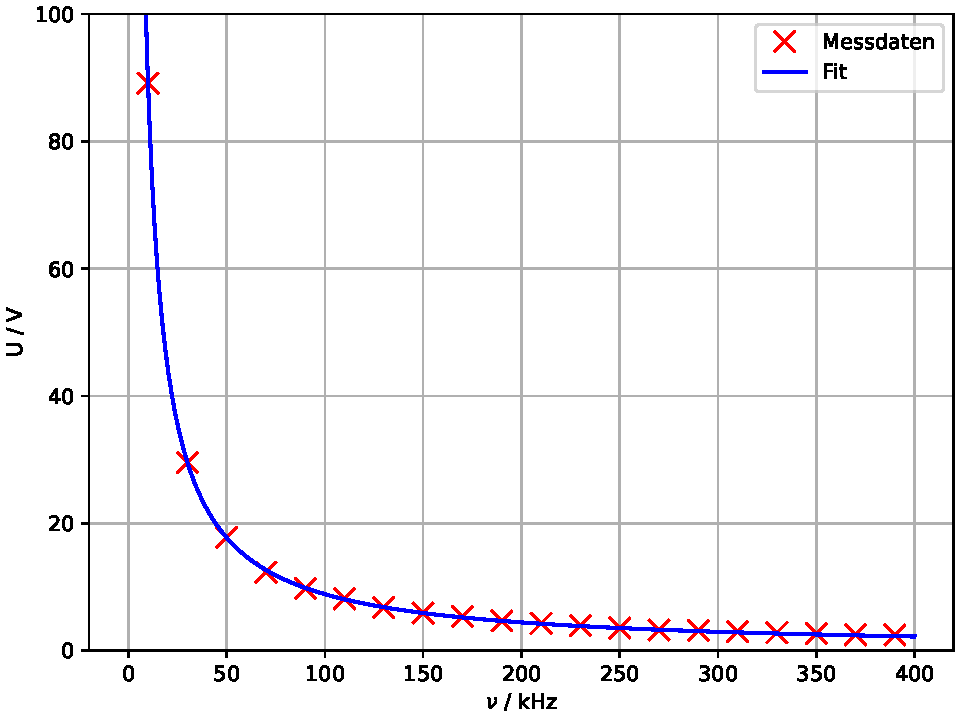
\includegraphics[height=6cm]{python/plota.pdf}
    \caption{Bereich von $30$ bis $1000 mbar$}
    \label{fig:MesswerteKlein}
  \end{subfigure}
  \hfill
  \begin{subfigure}{0.48\textwidth}
    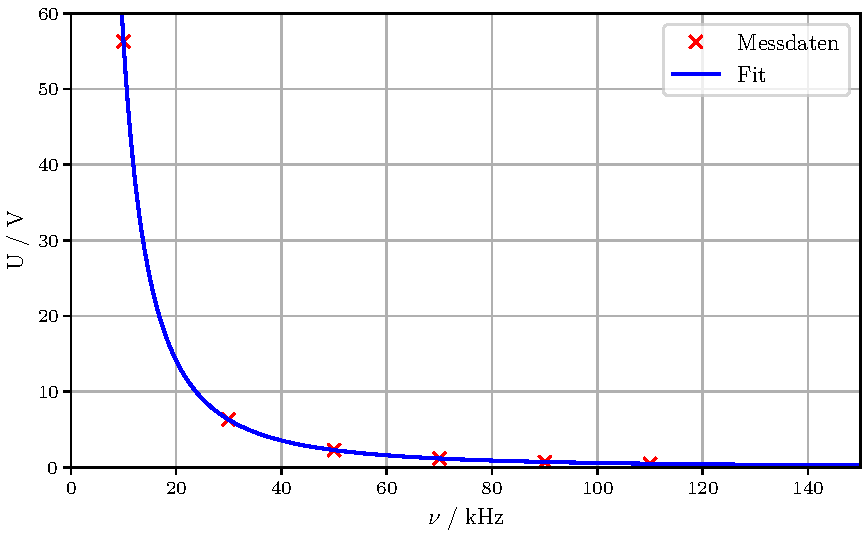
\includegraphics[height=6cm]{python/plotb.pdf}
    \caption{Bereich von $1$ bis $15 bar$}
    \label{fig:MesswerteGross}
  \end{subfigure}
  \caption{Die Messwerte der ersten Messreihe aufgetragen als der Logarithmus des Drucks $p$
  gegen die reziproke absolute Temperatur $T$.}
  \label{fig:Teila}
\end{figure}
\newpage
Um hier raus die Verdampfungswärme von Wasser zu bestimmen, legt man eine Gerade durch die Messwerte.
Diese wird mittels Python für den Bereich von $30$ bis $1000 mbar$ erstellt und sieht folgendermaßen aus: \\
\begin{figure}[H]
  \centering
  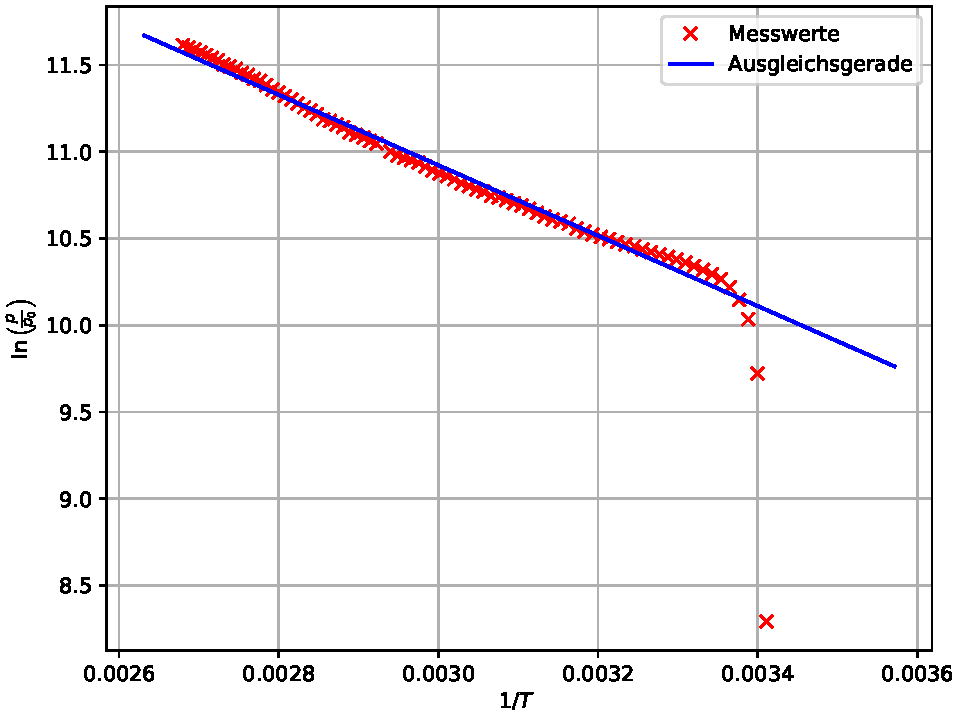
\includegraphics[width=\textwidth]{python/plotc}
  \caption{Die Messwerte der zweiten Messreihe aufgetragen als der Logarithmus des Drucks $p$
  gegen die reziproke absolute Temperatur $T$ mit der Ausgleichsgerade.}
  \label{fig:Ausgleichsgerade}
\end{figure}
Für diesen Fit wurden die ersten zwei Messwerte dieser Reihe nicht berücksichtigt, da diese die Bestimmung von $L$
offensichtlich verfälschen würden.
Die Gleichung des zu der Ausgleichsgerade ist:
\begin{equation}
  ln(p) = - \frac{L}{R} \cdot \frac{1}{T}
  \Rightarrow y = a \cdot x + b = -2029 * x + 17.010
\end{equation}
Mit Numerik Python ergeben sich folgende Messunsicherheiten: $a = \SI{-2029 \pm 21 }{\frac{1}{\kelvin}}$
und $b = \SI{17.010 \pm 0.063}{\frac{1}{\kelvin}}$
Für die Verdampfungswärme von Wasser ergibt sich zu
\begin{equation*}
  L = - \ a \cdot R \Rightarrow L = \SI{16870.1 \pm 174.6}{\frac{\J}{\mol}}
\end{equation*}
L ist die Steigung der Ausgleichsgeraden in Abbildung \ref{fig:Ausgleichsgerade} multipliziert mit der Universellen Gaskonstante R.

Nun folgt die Bestimmung der äußeren Verdampfungswärme $L_a$.
Diese beschreibt die benötigte Arbeit, um bei konstantem Druck das Volumen eines Stoffs zu verändern.
Hierfür wird die ideale Gasgleichung mit der verrichteten Arbeit gleich gesetzt.
\begin{equation}
    W = P \cdot V = R \cdot T = L_a
\end{equation}
Also ergibt sich $L_a = \SI{3101.3}{\frac{\J}{\mol}}$.
Um jetzt noch die erforderliche Arbeit zu Überwindung der molekularen Anziehungskraft bei Verdampfung $L_i$ zu bestimmen, wird
    die Differenz zwischen $L$ und $L_a$ gebildet.
\begin{equation}
    L_i = L - L_a \Rightarrow L_i = \SI{13768.8 \pm 174.6}{\frac{\J}{\mol}}
\end{equation}


% Siehe \autoref{fig:plot} und \autoref{tab:tabelle}!
\newpage
\subsection{d) Druck über einem Bar}
Auflösen er Clausius-Clapeyronschen Gleichung nach $L$ zur Bestimmung der Wärmeabhängigkeit.\\
\begin{align}
  &(V_D-V_F)dp=\frac{L}{T}dT\nonumber\\
  \Leftrightarrow L=&(V_D-V_F)\frac{dp}{dT}T
\end{align}
Errechnet man mittels Python und scipy einen polynomialen Fit vierten Grades, erhält das Polynom $ax^4+bx^3+cx^2+dx+e$ folgende Werte:
\begin{align*}
a = -0.000000000000003 ± 0.000000000000001\\
b = 0.000000000097499 ± 0.000000000026259\\
c = -0.000001522301035 ± 0.000000283848956\\
d = 0.015382375751184 ± 0.001167777905221\\
e = 377.748401598401188 ± 1.450339506446900
\end{align*}
\begin{figure}[h]
    \centering
    \includegraphics[height=8cm]{plot2.pdf}
    \caption{Druck und Temperatur der zweiten Messreihe, $p\geq 1$Bar.}
\end{figure}
\\
Ableitung des Polynoms
\begin{align}
T(p)&=-\num{3e-15}p^4+\num{9.75e-11}p^3-\num{1.522e-6}p^2+0,015p+377,748:\nonumber\\
T'(p)&=-\num{1.2e-14}p^3+\num{2.925e-10}p^2-\num{3.044}p+0,015
\end{align}
Das ist nun unser Asudruck für $\frac{dp}{dT}$.
